\documentclass[]{article}
\usepackage{lmodern}
\usepackage{amssymb,amsmath}
\usepackage{ifxetex,ifluatex}
\usepackage{fixltx2e} % provides \textsubscript
\ifnum 0\ifxetex 1\fi\ifluatex 1\fi=0 % if pdftex
  \usepackage[T1]{fontenc}
  \usepackage[utf8]{inputenc}
\else % if luatex or xelatex
  \ifxetex
    \usepackage{mathspec}
  \else
    \usepackage{fontspec}
  \fi
  \defaultfontfeatures{Ligatures=TeX,Scale=MatchLowercase}
\fi
% use upquote if available, for straight quotes in verbatim environments
\IfFileExists{upquote.sty}{\usepackage{upquote}}{}
% use microtype if available
\IfFileExists{microtype.sty}{%
\usepackage{microtype}
\UseMicrotypeSet[protrusion]{basicmath} % disable protrusion for tt fonts
}{}
\usepackage[margin=1in]{geometry}
\usepackage{hyperref}
\hypersetup{unicode=true,
            pdftitle={Vizualizace dat},
            pdfauthor={Irina Georgievová},
            pdfborder={0 0 0},
            breaklinks=true}
\urlstyle{same}  % don't use monospace font for urls
\usepackage{color}
\usepackage{fancyvrb}
\newcommand{\VerbBar}{|}
\newcommand{\VERB}{\Verb[commandchars=\\\{\}]}
\DefineVerbatimEnvironment{Highlighting}{Verbatim}{commandchars=\\\{\}}
% Add ',fontsize=\small' for more characters per line
\usepackage{framed}
\definecolor{shadecolor}{RGB}{248,248,248}
\newenvironment{Shaded}{\begin{snugshade}}{\end{snugshade}}
\newcommand{\KeywordTok}[1]{\textcolor[rgb]{0.13,0.29,0.53}{\textbf{#1}}}
\newcommand{\DataTypeTok}[1]{\textcolor[rgb]{0.13,0.29,0.53}{#1}}
\newcommand{\DecValTok}[1]{\textcolor[rgb]{0.00,0.00,0.81}{#1}}
\newcommand{\BaseNTok}[1]{\textcolor[rgb]{0.00,0.00,0.81}{#1}}
\newcommand{\FloatTok}[1]{\textcolor[rgb]{0.00,0.00,0.81}{#1}}
\newcommand{\ConstantTok}[1]{\textcolor[rgb]{0.00,0.00,0.00}{#1}}
\newcommand{\CharTok}[1]{\textcolor[rgb]{0.31,0.60,0.02}{#1}}
\newcommand{\SpecialCharTok}[1]{\textcolor[rgb]{0.00,0.00,0.00}{#1}}
\newcommand{\StringTok}[1]{\textcolor[rgb]{0.31,0.60,0.02}{#1}}
\newcommand{\VerbatimStringTok}[1]{\textcolor[rgb]{0.31,0.60,0.02}{#1}}
\newcommand{\SpecialStringTok}[1]{\textcolor[rgb]{0.31,0.60,0.02}{#1}}
\newcommand{\ImportTok}[1]{#1}
\newcommand{\CommentTok}[1]{\textcolor[rgb]{0.56,0.35,0.01}{\textit{#1}}}
\newcommand{\DocumentationTok}[1]{\textcolor[rgb]{0.56,0.35,0.01}{\textbf{\textit{#1}}}}
\newcommand{\AnnotationTok}[1]{\textcolor[rgb]{0.56,0.35,0.01}{\textbf{\textit{#1}}}}
\newcommand{\CommentVarTok}[1]{\textcolor[rgb]{0.56,0.35,0.01}{\textbf{\textit{#1}}}}
\newcommand{\OtherTok}[1]{\textcolor[rgb]{0.56,0.35,0.01}{#1}}
\newcommand{\FunctionTok}[1]{\textcolor[rgb]{0.00,0.00,0.00}{#1}}
\newcommand{\VariableTok}[1]{\textcolor[rgb]{0.00,0.00,0.00}{#1}}
\newcommand{\ControlFlowTok}[1]{\textcolor[rgb]{0.13,0.29,0.53}{\textbf{#1}}}
\newcommand{\OperatorTok}[1]{\textcolor[rgb]{0.81,0.36,0.00}{\textbf{#1}}}
\newcommand{\BuiltInTok}[1]{#1}
\newcommand{\ExtensionTok}[1]{#1}
\newcommand{\PreprocessorTok}[1]{\textcolor[rgb]{0.56,0.35,0.01}{\textit{#1}}}
\newcommand{\AttributeTok}[1]{\textcolor[rgb]{0.77,0.63,0.00}{#1}}
\newcommand{\RegionMarkerTok}[1]{#1}
\newcommand{\InformationTok}[1]{\textcolor[rgb]{0.56,0.35,0.01}{\textbf{\textit{#1}}}}
\newcommand{\WarningTok}[1]{\textcolor[rgb]{0.56,0.35,0.01}{\textbf{\textit{#1}}}}
\newcommand{\AlertTok}[1]{\textcolor[rgb]{0.94,0.16,0.16}{#1}}
\newcommand{\ErrorTok}[1]{\textcolor[rgb]{0.64,0.00,0.00}{\textbf{#1}}}
\newcommand{\NormalTok}[1]{#1}
\usepackage{longtable,booktabs}
\usepackage{graphicx,grffile}
\makeatletter
\def\maxwidth{\ifdim\Gin@nat@width>\linewidth\linewidth\else\Gin@nat@width\fi}
\def\maxheight{\ifdim\Gin@nat@height>\textheight\textheight\else\Gin@nat@height\fi}
\makeatother
% Scale images if necessary, so that they will not overflow the page
% margins by default, and it is still possible to overwrite the defaults
% using explicit options in \includegraphics[width, height, ...]{}
\setkeys{Gin}{width=\maxwidth,height=\maxheight,keepaspectratio}
\IfFileExists{parskip.sty}{%
\usepackage{parskip}
}{% else
\setlength{\parindent}{0pt}
\setlength{\parskip}{6pt plus 2pt minus 1pt}
}
\setlength{\emergencystretch}{3em}  % prevent overfull lines
\providecommand{\tightlist}{%
  \setlength{\itemsep}{0pt}\setlength{\parskip}{0pt}}
\setcounter{secnumdepth}{5}
% Redefines (sub)paragraphs to behave more like sections
\ifx\paragraph\undefined\else
\let\oldparagraph\paragraph
\renewcommand{\paragraph}[1]{\oldparagraph{#1}\mbox{}}
\fi
\ifx\subparagraph\undefined\else
\let\oldsubparagraph\subparagraph
\renewcommand{\subparagraph}[1]{\oldsubparagraph{#1}\mbox{}}
\fi

%%% Use protect on footnotes to avoid problems with footnotes in titles
\let\rmarkdownfootnote\footnote%
\def\footnote{\protect\rmarkdownfootnote}

%%% Change title format to be more compact
\usepackage{titling}

% Create subtitle command for use in maketitle
\newcommand{\subtitle}[1]{
  \posttitle{
    \begin{center}\large#1\end{center}
    }
}

\setlength{\droptitle}{-2em}
  \title{Vizualizace dat}
  \pretitle{\vspace{\droptitle}\centering\huge}
  \posttitle{\par}
  \author{Irina Georgievová}
  \preauthor{\centering\large\emph}
  \postauthor{\par}
  \predate{\centering\large\emph}
  \postdate{\par}
  \date{20.2.2017}

\usepackage[czech]{babel}

\usepackage{amsthm}
\newtheorem{theorem}{Theorem}[section]
\newtheorem{lemma}{Lemma}[section]
\theoremstyle{definition}
\newtheorem{definition}{Definition}[section]
\newtheorem{corollary}{Corollary}[section]
\newtheorem{proposition}{Proposition}[section]
\theoremstyle{definition}
\newtheorem{example}{Example}[section]
\theoremstyle{remark}
\newtheorem*{remark}{Remark}
\begin{document}
\maketitle

{
\setcounter{tocdepth}{2}
\tableofcontents
}
\section*{Praktická část}\label{prakticka-cast}
\addcontentsline{toc}{section}{Praktická část}

\section*{Základní grafy v R}\label{zakladni-grafy-v-r}
\addcontentsline{toc}{section}{Základní grafy v R}

Grafy jsou silnou stránkou R. Pro vytváření základních grafů v R
používáme vestavěný balíček \texttt{graphics}\footnote{\url{https://stat.ethz.ch/R-manual/R-devel/library/graphics/html/graphics-package.html}},
který obsahuje mnoho užitečných funkcí pro tvorbu grafických prvků.
První kapitola se soustředí na tyto funkce tohoto balíčku a v dalších
kapitolách jsou popsány funkce balíčků dalších (například
\texttt{lattice}, \texttt{ggplot2},\ldots{}), které zastávají podobné
funkce, avšak s různým rozsahem nastavení.\footnote{R Cookbook by Paul
  Teetor, p.221}

V následujících příkladech nejsou grafy doplněny o barvy, popisky os,
legendy ani názvy a především proto, že záměrem této kapitoly je popsat
základní grafy a funkce pro jejich tvorbu v prostředí R. Všechny tyto
prvky mohou být přidány do grafu, ale tím by příkazy obsahovali
irelevantní parametry vzhledem k zaměření této kapitoly. Základní funkce
\texttt{plot(x)} jejímž voláním se obdrží pole s grafickou reprezentaci
proměnné ``x'', by při doplnění kódu o veškeré paramtery vypadala
následovaně:\footnote{R Cookbook by Paul Teetor, p.221}:

\begin{Shaded}
\begin{Highlighting}[]
\KeywordTok{plot}\NormalTok{(x, }\DataTypeTok{main =} \StringTok{"Název grafu"}\NormalTok{, }\DataTypeTok{xlab =} \StringTok{"popis osy x"}\NormalTok{, }\DataTypeTok{ylab =} \StringTok{"popis osy y"}\NormalTok{, }
\OperatorTok{+}\StringTok{    }\DataTypeTok{col =} \KeywordTok{c}\NormalTok{(}\StringTok{"red"}\NormalTok{, }\StringTok{"black"}\NormalTok{, }\StringTok{"green"}\NormalTok{)) }
\end{Highlighting}
\end{Shaded}

Záměrem je tedy používání příkazů s pouze relevantními parametry.

\subsection{1.1. Bodový graf}\label{bodovy-graf}

Bodový graf je rychlým způsobem, jak znázornit vztahy a souvislosti mezi
proměnnými datasetu případně k zjištění jejich neexistence. Data jsou
zobrazeny v kartézském souřadném systému a mají pro každou hodnotu
proměnné danné místo na vodorovné a svislé ose. V případě existence
závislostí mezi proměnnými lze tuto závislost interpolovat přímkou,
křivkou či případně dalším vhodným vyobrazením této závislosti.

Pro vytvoření bodového grafu v základním prostředí R (pomocí
\texttt{graphics}) použijeme funkci \texttt{plot()}, která má tento typ
grafu předdefinovaný pro numerické hodnoty. Viz obrázek 1 (a). Nečiselná
data vytvoří jiný typ grafu. \footnote{\url{http://stat.ethz.ch/R-manual/R-devel/library/datasets/html/cars.html}}

\begin{Shaded}
\begin{Highlighting}[]
\KeywordTok{plot}\NormalTok{(cars)}
\end{Highlighting}
\end{Shaded}

\subsection{1.2. Liniový graf}\label{liniovy-graf}

Jediný rozdíl mezi bodovým a liniovým grafem je, že jeden zobrazuje body
a druhý je spojuje.\footnote{R Cookbook by Paul Teetor, p.241} (viz.
\autoref{fig1}) Pro vykreslení liniového grafu se používá již několikrát
zmíněná funkce \texttt{plot()}, kterou doplníme o požadovaný typ
vykreslení:

\begin{Shaded}
\begin{Highlighting}[]
\KeywordTok{plot}\NormalTok{(x, }\DataTypeTok{type=}\StringTok{"l"}\NormalTok{)}
\end{Highlighting}
\end{Shaded}

V tabulce \ref{tab:1} jsou uvedený některé základní atributy parametru
\texttt{type}, které můžeme použít\footnote{\url{https://stat.ethz.ch/R-manual/R-devel/library/graphics/html/plot.html}}:

\begin{longtable}[]{@{}ccc@{}}
\caption{\label{tab:1}: Základní atributy parametru
\texttt{type}}\tabularnewline
\toprule
& Anglický popis & Český popis\tabularnewline
\midrule
\endfirsthead
\toprule
& Anglický popis & Český popis\tabularnewline
\midrule
\endhead
p & points & bodový\tabularnewline
l & lines & liniový\tabularnewline
b & both & složený\tabularnewline
h & histogram & histogram\tabularnewline
n & no plotting & bez vykreslení\tabularnewline
\bottomrule
\end{longtable}

\begin{figure}

{\centering 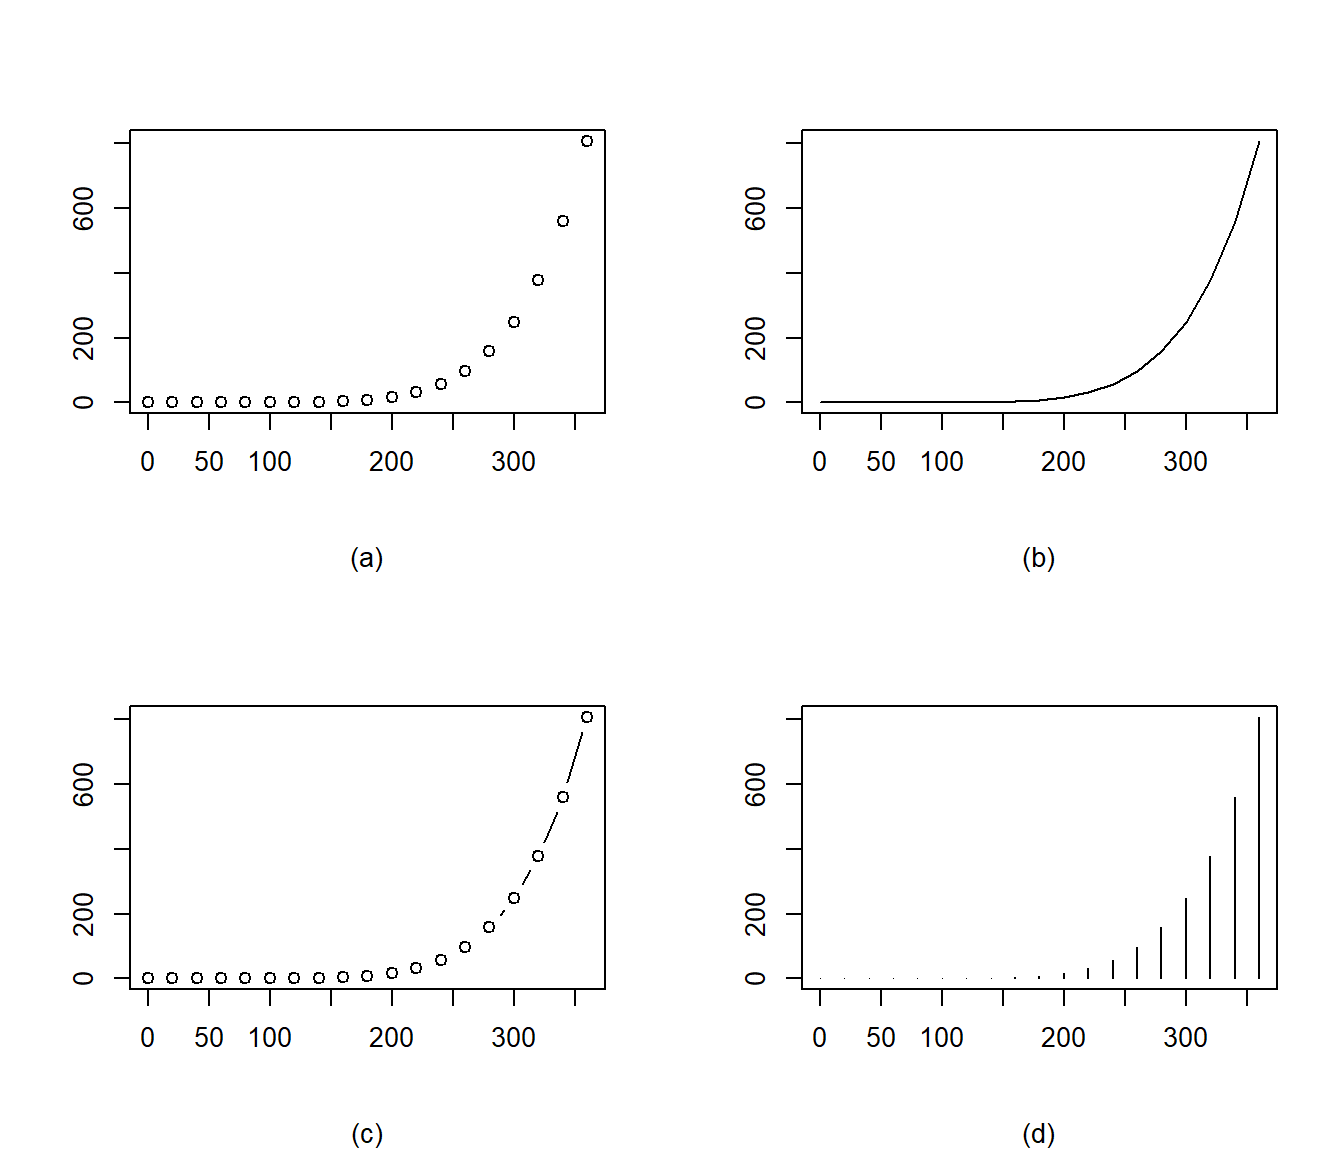
\includegraphics{Chapter_1_files/figure-latex/graf_typy-1} 

}

\caption{\label{fig1}Porovnání základních typů grafů}(\#fig:graf_typy)
\end{figure}

Popis a všechny atributy dalších parametrů funkce \texttt{plot()} lze
nálézt v nápovědě zadáním příkazu \texttt{?plot()}.

\newpage

\subsection{1.3. Sloupcový graf}\label{sloupcovy-graf}

Sloupcový graf je možná nejvíce používaným způsobem vizualizace dat.
Obvykle se používá pro zobrazení číselných hodnot na ose y pro různé
kategorie na ose x. Výška sloupců může reprezentovat jak četnosti
výskytu hodnot, tak i samotné hodnoty.\footnote{R Graphics Cookbook by
  Winston Chang, p.19} V R lze tento typ grafu vykreslit pomocí funkce
\texttt{barplot()}. V příkladu je použit data set \texttt{mtcars},
konkretně atribut \texttt{cyl}- počet válců v motoru.

\begin{Shaded}
\begin{Highlighting}[]
\KeywordTok{table}\NormalTok{(mtcars}\OperatorTok{$}\NormalTok{cyl)}
\end{Highlighting}
\end{Shaded}

\begin{verbatim}
## 
##  4  6  8 
## 11  7 14
\end{verbatim}

\begin{Shaded}
\begin{Highlighting}[]
\KeywordTok{barplot}\NormalTok{(}\KeywordTok{table}\NormalTok{(mtcars}\OperatorTok{$}\NormalTok{cyl))}
\end{Highlighting}
\end{Shaded}

\begin{center}\includegraphics[width=0.5\linewidth]{Chapter_1_files/figure-latex/unnamed-chunk-4-1} \end{center}

\subsubsection{1.3.1. Histogram}\label{histogram}

Sloupcový graf s četnostmi na souvislé ose je taky známý jako
histogram.\footnote{R Graphics Cookbook by Winston Chang, p.26} Četnosti
mohou být absolutní či relativní. Absolutní četnost (nebo jen četnost
třídy) zobrazuje počet statistických jednotek s hodnotou znaku, který
patří do určité třídy. Podíl příslušné četnosti a rozsahu datového
souboru se nazývá relativní četnost.\footnote{PRAVDĚPODOBNOST A
  MATEMATICKÁ STATISTIKA by Doc. RNDr. Jana Novovičová, CSc., p.15}
Šířka sloupce reprezentuje jednotlivé intervaly, které mají stejnou
délku. Pro výpočet optimální délky intervalu existují různé metody.
Základní histogram se vytváří pomocí funkci \texttt{hist()} a její
atribut \texttt{breaks} udává buď hranice intervalů, jejich preferovaný
počet nebo metodu výpočtu intervalu. V R jsou vestavěny 3 metody
výpočtu\footnote{Data Representations, Transformations, and Statistics
  for Visual Reasoning by Ross Maciejewski, p.18}:

\begin{enumerate}
\def\labelenumi{\arabic{enumi}.}
\tightlist
\item
  Sturges
\end{enumerate}

\begin{Shaded}
\begin{Highlighting}[]
\KeywordTok{hist}\NormalTok{(x, }\DataTypeTok{breaks =} \StringTok{"Sturges"}\NormalTok{)}
\end{Highlighting}
\end{Shaded}

\[k=[log_2(n)]+1\] Kde \(k\) je počet intervalů a \(n\) je počet prvků
případně počet pozorování výběru \(x\). Délka intervalu se tedy získá
jako \(h=(\max(x)-\min(x))/k\). Tato metoda je výchozí pro funkci
\texttt{hist()}.

\begin{enumerate}
\def\labelenumi{\arabic{enumi}.}
\setcounter{enumi}{1}
\tightlist
\item
  Scott
\end{enumerate}

\begin{Shaded}
\begin{Highlighting}[]
\KeywordTok{hist}\NormalTok{(x, }\DataTypeTok{breaks =} \StringTok{"Scott"}\NormalTok{)}
\end{Highlighting}
\end{Shaded}

Počet intervalů může být přidělen přímo nebo může být vypočítán z
předpokládané šířky intervalu \(h\):
\[k=\Big[\frac{max(x)-min(x)}{h}\Big]\] Scotovo pravidlo je následující:
\[h=\frac{3.5\sigma}{n^{\frac{1}{3}}}\] Případně oba vztahy lze shrnout
do jednoho:
\[k = \Big[n^{\frac{1}{3}}{\frac{max(x)-min(x)}{3.5\sigma}}\Big]\]

kde \(\sigma\) je směrodatná odchylka.

\begin{enumerate}
\def\labelenumi{\arabic{enumi}.}
\setcounter{enumi}{2}
\tightlist
\item
  Freedman-Diaconic
\end{enumerate}

\begin{Shaded}
\begin{Highlighting}[]
\KeywordTok{hist}\NormalTok{(x, }\DataTypeTok{breaks =} \StringTok{"FD"}\NormalTok{)}
\end{Highlighting}
\end{Shaded}

\[h=2\frac{IQR(x)}{n^{\frac{1}{3}}}\] Po upravě:
\[k = \Big[n^{\frac{1}{3}}{\frac{max(x)-min(x)}{2IQR(x)}}\Big]\] \(IQR\)
je mezikvartilové rozpětí, které definujeme jako rozdíl 75\% a 25\%
kvantilů.

Histogram se používá většinou pro spojitá data (Graf 2), ale může být
použit i pro diskrétní (Graf 1), viz. kapitola XX.

\begin{center}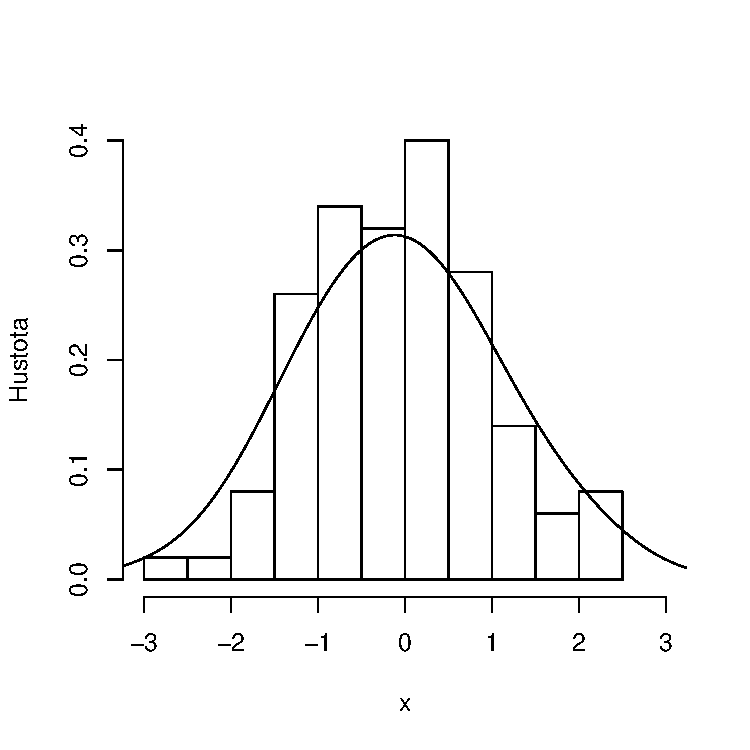
\includegraphics{Chapter_1_files/figure-latex/hist_example-1} \end{center}

\subsubsection{1.3.2. Koláčový graf}\label{kolacovy-graf}

Koláčový graf představuje plný kruh (360°), který je rozdělen na
jednotlive výseče pro znázornění číselných proporci mezi proměnnými.
Koláčový graf je tvořen transformaci skládanýho sloupcového grafu do
polárního souřadnicového systému.\footnote{Leland Wilkinson, The Grammar
  of Graphics, p.207}

\begin{center}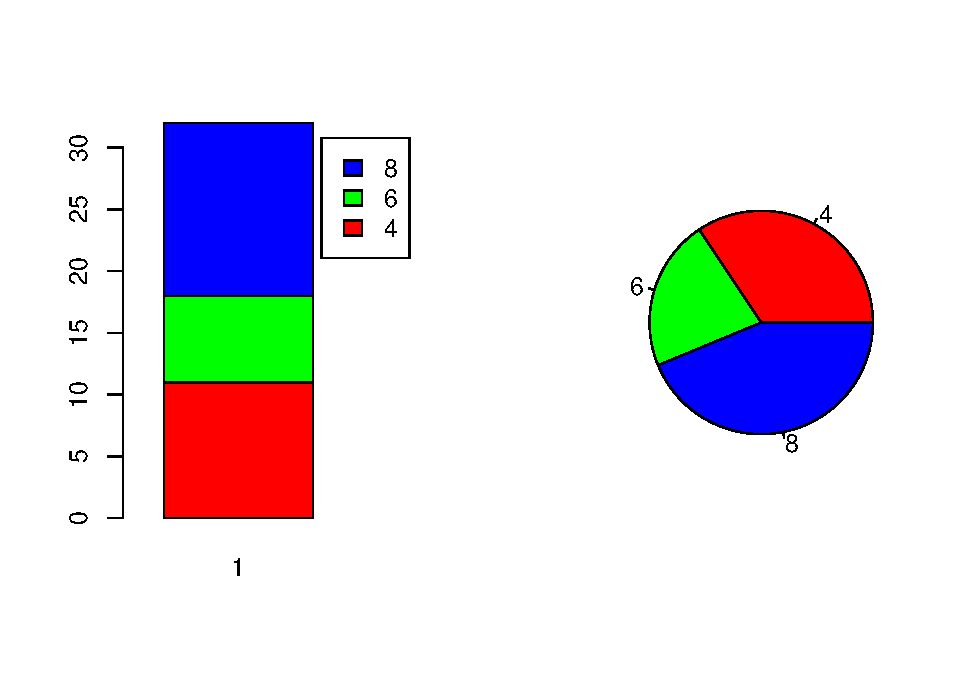
\includegraphics[width=0.7\linewidth]{Chapter_1_files/figure-latex/barplot_to_pie-1} \end{center}

Koláčové grafy mohou být jednoduché, s vysvětlivkami, 3D. Jednoduché
koláčové grafy se výkreslují pomoci funkci \texttt{pie()}. Požadovaným
vstupem pro základní výkreslení grafu je vektor kladných čísel, atributy
\texttt{labels} (popisky), \texttt{col} (barvy), \texttt{main}
(titulek), \texttt{radius} (poloměr), \texttt{clockwise} (směr
výkreslení) atd. jsou pouze doplňkovými.

\begin{Shaded}
\begin{Highlighting}[]
\KeywordTok{pie}\NormalTok{(x, labels, col, main, radius, clockwise)}
\end{Highlighting}
\end{Shaded}

\begin{center}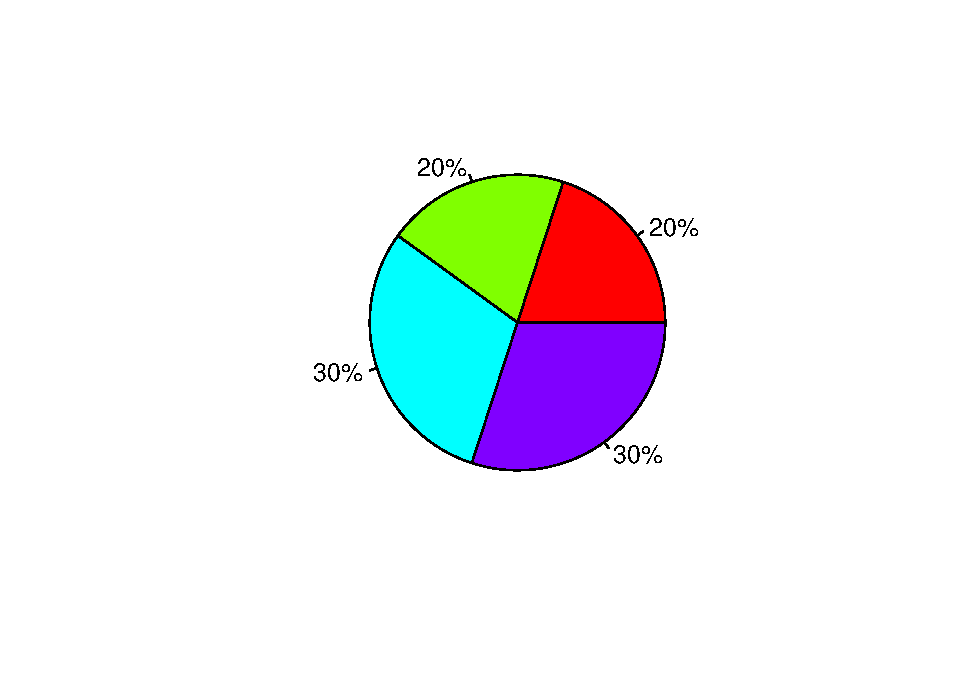
\includegraphics[width=0.75\linewidth]{Chapter_1_files/figure-latex/pie_example-1} \end{center}

Koláčové grafy se mnohdy používají nekorektně, vnímání takových grafu je
obtížné. Následující graf je takovým příkladem.

\begin{center}\includegraphics[width=0.75\linewidth]{Chapter_1_files/figure-latex/pie_3D-1} \end{center}

Jednotlivé kategorie tohoto grafu mají podobné procentuální zastoupení,
ale protože modrá výseč se nachází nejblíž, vnímá se jako dominantní.
Přestože tento příklad se považuje za extrémní, 3D koláčové grafy i s
malým počtem kategorii se těžce rozlišují.

Další častou chybou je nekorektní význačení procentuálního zastoupení
jednotlivých kategorii. ??

\subsection{1.4. Krabicový graf}\label{krabicovy-graf}

Krabicový graf poskytuje rychlé a jednoduché vizuální srhnití datasetu.
V balíčku \texttt{grafics} funkcí, kterou vytvaří tento typ grafů je
\texttt{boxplot(x)}. Obrázek X znázorňuje typycký krabicový graf, kde
silná čára uprostřed je medián, ``krabice'' kolem ní určuje polohu
prvního a třetího kvartilů (dolní je Q1 a horní je Q3). ``Ocásky'' nad a
pod krabici znázorňují rozpětí dat, nepočítaje odlehlé hodnoty.

\begin{Shaded}
\begin{Highlighting}[]
\KeywordTok{boxplot}\NormalTok{(x)}
\end{Highlighting}
\end{Shaded}

\includegraphics{Chapter_1_files/figure-latex/unnamed-chunk-7-1.pdf}


\end{document}
